%
% File acl2019.tex
%
%% Based on the style files for ACL 2018, NAACL 2018/19, which were
%% Based on the style files for ACL-2015, with some improvements
%%  taken from the NAACL-2016 style
%% Based on the style files for ACL-2014, which were, in turn,
%% based on ACL-2013, ACL-2012, ACL-2011, ACL-2010, ACL-IJCNLP-2009,
%% EACL-2009, IJCNLP-2008...
%% Based on the style files for EACL 2006 by 
%%e.agirre@ehu.es or Sergi.Balari@uab.es
%% and that of ACL 08 by Joakim Nivre and Noah Smith

\documentclass[11pt,a4paper]{article}
\usepackage[hyperref]{acl2019}
\usepackage{times}
\usepackage{latexsym}
\usepackage{graphicx}
\usepackage{siunitx}
\usepackage{subfig}

\usepackage{multicol}
\usepackage{url}

\aclfinalcopy % Uncomment this line for the final submission
%\def\aclpaperid{***} %  Enter the acl Paper ID here

%\setlength\titlebox{5cm}
% You can expand the titlebox if you need extra space
% to show all the authors. Please do not make the titlebox
% smaller than 5cm (the original size); we will check this
% in the camera-ready version and ask you to change it back.
\newcommand\BibTeX{B\textsc{ib}\TeX}
\title{Defining and predicting hydrophobic areas on protein surfaces}
\author{Jan van Eck\\
    Student number: 2563960\\
  Bioinformatics and System Biology at Vrije Universiteit Amsterdam \\
  \texttt{janvaneck94@gmail.com} \\\
  \\
  Supervisors:\\
  Sanne Abeln, Juami van Gils\\
  \\
  Course ID: XM\_0070\\
  Credit points: 36ECTs
  
%   And
%   Second Author \\
%   Affiliation / Address line 1 \\
%   Affiliation / Address line 2 \\
%   Affiliation / Address line 3 \\
%   \texttt{email@domain} \\
}



\begin{document}
\maketitle



\clearpage
\begin{abstract}
  In general, hydrophobic residues tend to be buried in the interior of a protein to avoid contact with a hydrophilic solvent. Nevertheless, large hydrophobic areas can be found on a protein’s surface. The size of the hydrophobic surface area and, more specifically, hydrophobic patches play essential roles in protein-protein interactions or non-specific aggregation. In the absence of structural information, the prediction of the size of the solvent-accessible hydrophobic area and patches is, therefore, valuable for deciphering its function. In this work, we present simple methods for predicting the total hydrophobic surface area and relative hydrophobic surface area of a protein. The methods were benchmarked against NetSurfP2. We show that solely NetSurfP2 results are a good estimator for the hydrophobic surface area. Furthermore, we present MolPatch: a method to calculate the hydrophobic patches of a protein from structural data. The three largest hydrophobic patches obtained with MolPatch contained a significant increase in protein interaction sites compared to random patches. We also show that the size of the largest patch can be predicted from the sequence with reasonable accuracy. These predictions can lead to a better understanding of the role of a protein's hydrophobic surface area in the context of protein-protein interactions, non-specific aggregation, and misfolding.
\end{abstract}
\section{Introduction}
Most proteins have hydrophobic residues that interact with each other. Upon folding in a aqueous environment, this results in a protein conformation where hydrophobic residues favor to be buried. This effect is known as ‘hydrophobic collapse’  \cite{dill1985theory}. The expectation is that hydrophobic residues of a protein are located at its core. Nevertheless, these residues can be found outside of the core, resulting in exposed unfavorable hydrophobic surface on proteins (Figure~\ref{hydrophhydrophil}A) \cite{van1995hydrophobicity,  kato1980hydrophobicity}.

The total hydrophobic surface area (THSA) (Figure~\ref{hydrophhydrophil}B) and relative hydrophobic surface area (RHSA)(Figure~\ref{hydrophhydrophil}C) play essential roles in a protein's function. Also, the size of large hydrophobic patches on the surface of the protein can influence its binding potential. The hydrophobic surface can affect protein-protein interactions \cite{larsen1998morphology}, non-specific aggregation \cite{beyreuther1991mechanisms}, and misfolding \cite{dobson2004principles}. Moreover, experimental techniques like electrophoresis \cite{wilkins1998two} and high-performance liquid chromatography \cite{kaliszan1990high} are based on the fact that some proteins have a larger hydrophobic surface area. The differences in hydrophobicity between proteins can have a direct impact on the outcomes of these experiments.

The number of known protein sequences and structures grows exponentially but not at the same rate. The PDB database provides structural information of 161,002 proteins \cite{berman2002protein}, while the UniProtKB/TrEMBL database contains 177,754,527 protein sequences \cite{uniprot2019uniprot}. The prediction of structural features from sequence could provide a solution to narrow the gap between the number of known protein sequences and known protein structure.

\begin{figure}[h!]
  \centering
  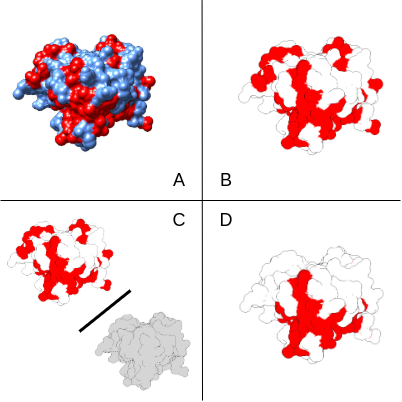
\includegraphics[width=0.4\textwidth]{figures/THSA_RHSA_LHPSA.png}
  \caption{The figure depicts the Chimera hydrophobicity surface representation of isomerase (PDB:3FZ5). The red color indicates the surface of hydrophobic residues, Blue indicates the surface of hydrophillic residues, and grey indicates the total surface area. Figure A shows that, although the surface of the protein mainly consists of hydrophilic sites, hydrophobic sites can also be observed on the surface. The total hydrophobic surface area (THSA) can be calculated by summing the area of all hydrophobic residues (figure B). The relative hydrophobic surface area (RHSA) can be calculated by deviding the THSA by the total surface area. The largest hydrophobic patch surface area is the largest area of adjacent hydrophobic residues (figure D)}
  \label{hydrophhydrophil}
\end{figure}

There are methods available to predict the accessible surface area (ASA) and relative surface area (RSA) of residues using solely the amino acid sequence \cite{klausen2019netsurfp, hanson2019improving, kallberg2014raptorx}. These methods use conservation data as input and deep neural networks for their predictions. Out of all the methods, NetSurfP2 is currently the best performing tool for ASA per residue prediction \cite{klausen2019netsurfp}. It uses an architecture composed of convolutional and long short-term memory neural networks trained on solved protein structures. It is possible to derive the THSA and RHSA from the  NetSurfP2 ASA per residue predictions. Although NetSurfP2 has high accuracy on these predictions, it does not necessarily mean it is a good predictor for THSA and RHSA. For example, Robbin Bouwmeester created a simple prediction model that outperformed NetSurfP1 \cite{petersen2009generic} in 2015.  Robbin Bouwmeester's model achieved a better performance because the nature of the prediction problem shifted from predicting the burial of a hydrophobic residue to the exposure of all residues.

No methods are currently available to predict the size of the largest hydrophobic patch surface area (LHPSA) (Figure~\ref{hydrophhydrophil}D) from a sequence. Quilt by Philip Lijnzaad \cite{lijnzaad1996method}, or the method by Eisenhaber and Argos \cite{eisenhaber1996hydrophobic} are already existing methods for determining the LHPSA using structural information such as PDB files. These methods detect hydrophobic patches based on the connection of surface-exposed areas. When looking for hydrophobic patches, carbon and sulfur atoms in the protein are often classified as hydrophobic. These methods show that interaction sites can be found on large hydrophobic patches using a small dataset of proteins \cite{lijnzaad1997hydrophobic}. A challenge in the detection of hydrophobic patches is accurately identifying and decoupling two seemingly separate patches that are connected with a small string of hydrophobic atoms \cite{lijnzaad1996method}. These so-called 'channels' are hard to detect using computer algorithms.

Given the importance of THSA, RHSA, and LHPSA on the molecular function of a protein two main questions arise. First, is it possible to improve the prediction of THSA and RHSA from sequence only? Second, is it possible to predict the LHPSA from sequence only?

 In order to  predict LHPSA, we also needed to create a stable definition of a hydrophobic patch. To this end, we created MolPatch. This is a method for determining hydrophobic patches based on PDB structures. MolPatch is initially based on currently existing hydrophobic patch detection algorithms but differs in the method for detaching patches connected by channels. Furthermore, simple models were trained to predict THSA, and RHSA directly from sequence and compare it with NetSurfP2 predictions. The result of this research shows that a simple model based on global features can not outperform NetSurfP2. We also trained multiple simple models to predict the LHPSA derived from MolPatch. The model whose accuracy turned out to be the highest, was trained with NetSurfP2 data.

\section{Methods}

To predict the THSA, RHSA, and LHPSA directly from a protein's sequence, the following steps were taken: The first step was to generate a PDB dataset to train and test our models. This step was followed up by determining the predictors. To calculate the LHPSA, we created MolPatch: a tool to determine hydrophobic patches on the surface of a protein. Protein interaction sites on hydrophobic patches were investigated by checking if protein interaction sites are often located on larger patches. The THSA and RHSA of proteins in the dataset could be resolved using DSSP. After calculating the predictors, global protein features were derived using the protein sequence, and different models were trained to predict the THSA, RHSA, and LHPSA. The THSA and RHSA models were benchmarked against each other and NetSurfP2. By lack of competitors, the predictive power of the LHPSA models was evaluated against a naive model.

\subsection{Datasets}
This study used Two datasets. The first dataset was culled with PISCES. PISCES is a public server for culling sets of protein sequences from the Protein Data Bank (PDB) by sequence identity and structural quality criteria \cite{wang2003pisces}. PISCES made it possible to construct a benchmark dataset with a predefined sequence identity cutoff, resolution cutoff in angstroms, and the R-factor. The chosen parameters were as follows: sequence percentage identity lower or equal to 25\%, resolution lower or equal to 3.0\si{\angstrom}, R-factor lower or equal to 0.3, sequence length within the range of 40-10,000 amino acids,  and non-X-ray entries and C$\alpha$-only entries were excluded. The culled dataset consisted of 13858 unique protein structures with a selection of 14604 chains. Two chains were removed from the dataset because the PDB files were obsolete. The dataset was filtered on monomer proteins, which resulted in a dataset of 5110 unique monomeric protein structures.

Transmembrane proteins have a relatively large hydrophobic surface area. This clashes with our model which was made for soluble proteins where hydrophobic residues tend to be buried. TMHMM was used to filter transmembrane protein from the dataset. TMHMM is a tool used to predict transmembrane protein based on the amino acid sequence \cite{sonnhammer1998hidden,moller2001evaluation}. The tool returns the expected number of amino acids in transmembrane helices. If this number is larger than 18, the protein was marked as a transmembrane protein and removed from the dataset. In total, 135 transmembrane monomers were removed from the dataset. The final dataset for training and testing of the models contained 4975 monomers.

A second dataset with information about protein binding sites was obtained via the PiSITE database. PiSITE provides information about the protein interaction sites of a protein. Both interaction information from a single PDB complex and interaction information between multiple PDBs are stored  \cite{higurashi2009pisite}. Only PiSITE information of the proteins from the original 14602 chains dataset was included in the dataset. The proteins without interaction sites and transmembrane proteins were filtered, which resulted in the final dataset of 4255 entries with information about protein interaction sites. This dataset was not filtered for monomers because a lot of the interaction sites were between chains in the same complex.

\subsection{Hydrophobic patch recognition using MolPatch}
MolPatch was created to detect hydrophobic patches on a protein surface using structural information from PDB. A patch is defined as a contiguous area of the solvent excluded surface (SES) of hydrophobic atoms. In this research, two methods to detect hydrophobic patches are proposed. The first method is an atom-based method where solely carbon and sulfur atoms were selected to be located in hydrophobic patches ($hydr_{atoms}$). 

\begin{equation}
hydr_{atoms} = \{carbon, sulfor\}
\end{equation}

It is possible to make a more sophisticated classification of $hydr_{atoms}$, but this is left out to keep the method less complicated and better interpretable. The second method is a residue-based method where only hydrophobic residues are allowed to be in hydrophobic patches. The hydrophobic residues ($hydr_{residues}$) are defined as:

\begin{equation}
hydr_{residues} = \{A, F, C, L, I, W, V, M, Y \}
\end{equation}

Note that the atom-based method does allow other residues than specified in $hydr$ to be located in a patch. The residue-based method only calculates patches containing residues from $hydr$.

\subsubsection{Specification of adjacent hydrophobic areas}
 The definition of adjacent hydrophobic areas should first be determined when searching for hydrophobic patches. One could, for example, determine adjacency by calculating the distance between the two centers of hydrophobic atoms or hydrophobic residues and determine if they are within a specific range from each other. Atoms or residues within this distance range could then be classified as adjacent. Figure \ref{fig2}A shows that this method can give incorrect results. Two atoms can, for example, be located within the adjacency search distance of the diameter of the atom, while the surface areas are not adjacent. Therefore, a more sophisticated technique is used by creating a solvent excluded surface (SES) point cloud using MSMS  \cite{sanner1996reduced}. This way, every atom on the surface is covered by multiple points (Figure \ref{fig2}B). With multiple points on one atom, a shorter adjacency search radius could be used. A solvent excluded surface is composed of the contact with a solvent molecule ("probe") rolling over the exposed atomic surface, toroidal, and reentrant surface. This is different from the solvent-accessible surface, where the center of the probe is traced. The SES for the residue and atom-based method was constructed using a probe of 1.5\si{\angstrom} and a density of 1.5 points per $\si{\angstrom}^2$.

Each point on the MSMS generated point surface was labeled hydrophobic or hydrophilic based on the hydrophobicity classification of the closest atom or residue depending on if the atom or residue-based method was used. Pairs of points were then created if the points existed within a range of 1.25\si{\angstrom} of each other. This search was performed with the KDTree algorithm to speed up the process \cite{bentley1975multidimensional}. Edges were created between hydrophobic labeled node pairs. This created a network of isolated hydrophobic patches. The individual network components were then extracted for accessible surface area estimation.

\begin{figure}[h!]
  \centering
  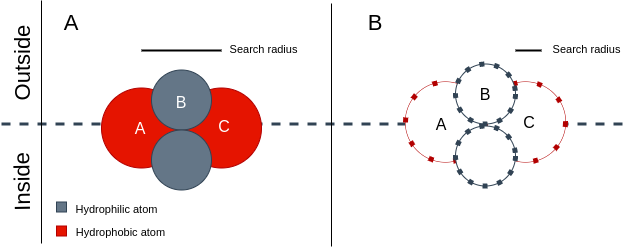
\includegraphics[width=0.48\textwidth]{figures/fig2.png}
  \caption{Figure A shows that hydrophobic atom A and C are within a pre-determined radius from each other. This radius would classify A and C as adjacent atoms while, in reality, atom B intersects the surface area of both atoms. Figure B represents a method were surface points are generated. Multiple dots are covering the surface area of an atom in the case of figure B. Due to the larger quantity of dots, a smaller adjacency search radius can be set.}
  \label{fig2}
\end{figure}

\subsubsection{Correction for the atom-based method}
An frequently encountered problem when defining hydrophobic patches is the connection of two separate patches by a thin string of hydrophobic atoms. A technique that has been proposed to adjust for this is the expansion of the hydrophobic atom probes (figure \ref{fig3}A) \cite{eisenhaber1996hydrophobic}. This method can correct for channels when the hydrophobic atoms are relatively low on the surface area, but cannot separate two networks connected by a line of hydrophobic atoms when this line lays higher on the surface than the surrounding hydrophilic atoms  (figure \ref{fig3}B).

\begin{figure}[h!]
  \centering
  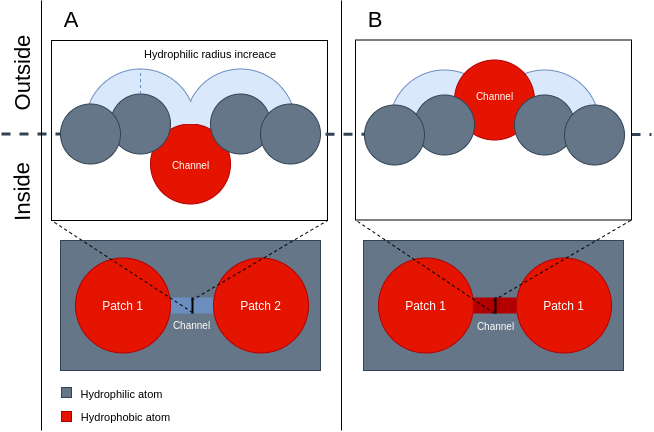
\includegraphics[width=0.48\textwidth]{figures/figure_draft_final2.png}
  \caption{In figure A, The atomic radius of the hydrophilic atoms is increased with respect to the original van der Waals radius. This results in the removal of the hydrophobic channel between two patches. Figure B shows the same channel, but the hydrophobic atoms lay higher on the surface than the hydrophilic. Expanding the radius will not remove the channel in this situation. Both channels are represented in the rectangle at the bottom of the figure. In figure A shows a channel removal by expanding the hydrophilic atoms. The rectangle in Figure B shows the same scenario without a channel cut off due to the higher located hydrophobic atom. This way, both patches stay adjacent to each other.
}
\label{fig3}
\end{figure}

The atom-based method is prone to the formation of channels (figure \ref{fig4}A). This problem of channel formation has been observed less in residue-based hydrophobic area selection, due to the broader area span of a residue (figure \ref{fig4}B). To reduce the amount of channels, we propose a straight forward method where edges are removed when one of the two closest atoms of a surface point is hydrophilic. The downside of this method is the unwanted loss of border areas in the patch. This border area loss also occurs when expanding hydrophilic atoms. A larger expansion radius causes an even more substantial unwanted loss.

\begin{figure}[h!]
  \centering
  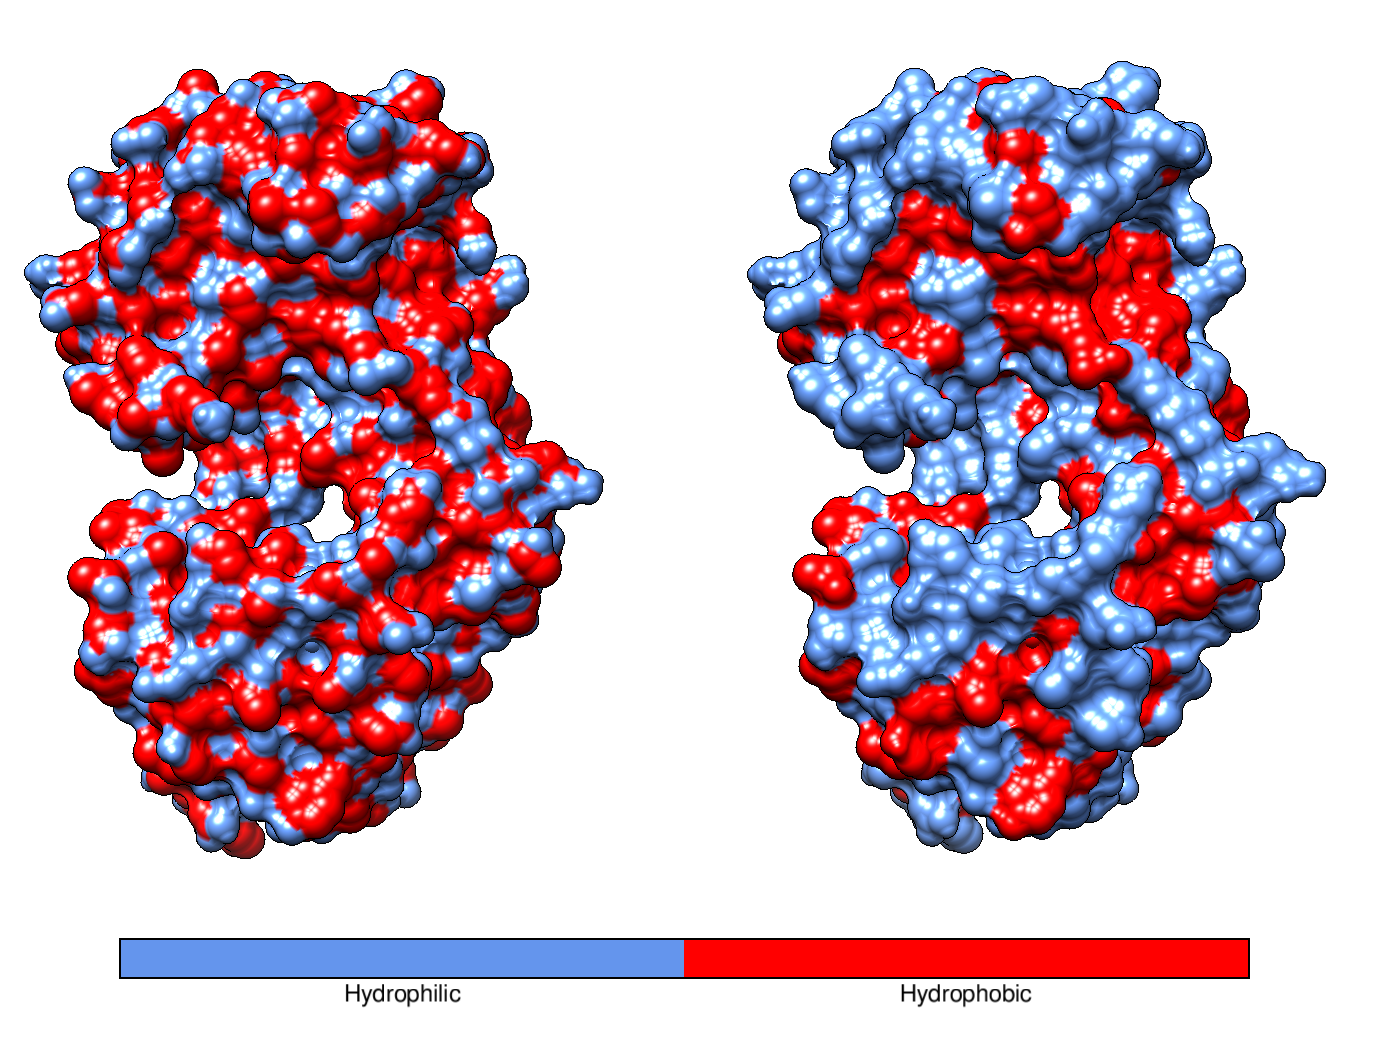
\includegraphics[width=0.48\textwidth]{figures/fig4.png}
  \caption{In figure A, an example of an atom-based hydrophobic SES assignment for Delta prime subunit (PDB:1A5TA). Without a correction by removing a large number of small channels between hydrophobic atoms, the largest hydrophobic patch covers the entire molecule. Figure B shows the residue-based hydrophobic SES assignment. A larger hydrophilic area compared to the atom-based method can be observed using this method.}
  \label{fig4}
\end{figure}

\subsubsection{Investigating the hydrophobic patches}
To investigate the biological relevance, the largest patches identified by MolPatch were analysed for protein interaction sites. For the top 20 largest patches detected by MolPatch, the total number of residues in the patch and the number of PiSITE corresponding residues in the patch were counted. In the case of the atom-based method, the residues that correspond to the atoms in the patch were counted. This results in the inclusion of a residue if only one atom participated in a patch and made it also possible for a residue to be located in multiple patches. The fraction of PiSITE residues in a patch was calculated to analyze if it exceeded random expectations. These random expectations were obtained by randomly selecting an equal amount of surface-exposed residues as initially observed in the patch. The fraction of interaction sites in the patch of randomly selected residues were then determined. The p-values from Wilcoxon tests were obtained on the difference between the fraction of protein interaction sites within a patch and the faction of protein interaction sites in the random selection. This tests were performed on the top 20 largest patches separately.


\subsection{Accessible surface area estimation}
The atom-based and residue-based methods both require different approaches when determining the ASA of the patches. FreeSASA was chosen to calculate the ASA for the atom-based approach \cite{mitternacht2016freesasa}. The ASA of a residue was assigned using DSSP \cite{kabsch1983dictionary} defaulting to the Sander and Rost maximum residue area values \cite{rost1994conservation}. The implementation of DSSP in the Biopython library was used for this task. If FreeSASA or DSSP were not able to resolve the ASA of a certain residue due to ambiguity, the residue was marked as an unknown residue. In case of an unknown residue with a known ASA, the ASA was added to the total accessible surface area but could never be added to the hydrophobic surface area. The same conversion to an X residue in the sequence happened to these cases.

\subsubsection{LHPSA calculation using the MolPatch atom and residue based method}
The atom-based method detects a patch in a way that all atoms located within a patch are known. The accessible surface area of all unique atoms in a patch was calculated using FreeSASA to estimate the size of the hydrophobic patch. The hydrophobic patch surface area using the atom-based method was estimated by summing the ASA of unique atoms in the patch. Patch size estimation using the residue-based method was performed using the DSSP library. The hydrophobic patch surface area was estimated by summing the DSSP derived ASA of each unique residue located in a patch. 

\subsubsection{THSA and RHSA calculation}
The total hydrophobic surface area THSA was calculated by summing the ASA of the residues of the protein, which belonged to a predefined set of hydrophobic amino acids hydr. The relative hydrophobic surface area RHSA was determined by dividing the THSA with the total accessible surface area. The total accessible surface area was determined by summing the ASA of all residues in a protein.

\subsection{The regression models used for predicting the THSA, RHSA, and LHPSA}
Different regression models were created to predict the THSA, RHSA, and LHPSA. In total, four distinct models were created, and one combination model.

\subsubsection{Naive length-based reference model}
A naive model was created to compare the relative performance of the other models. This simple model predicts the THSA, RHSA, or LHPSA based on the length of the sequence as a single feature. A simple linear regression was trained on this feature.

\subsubsection{Three Feature Model}
The three feature model (TFM) was created by Robin Bouwmeester in 2015 and performed best when predicting the THSA. This model was compared with NetSurfP1, which had the second-best performance. The TFM is a simple model with only three global features: sequence length, the number of hydrophilic, and hydrophobic amino acids of a protein. The Cubist regression in the CARET module was used as a training method.

\subsubsection{Global Feature Model}
The Global Feature Model (GFM) is a simple model that makes its predictions based on all global features obtained from the input sequence. In total, 31 global protein features were derived for prediction. The first 20 were the individual amino acid counts. Other features included were: length of the sequence, entropy,  hydrophobic amino acid count, polar amino acid count, molecular weight, aromaticity \cite{lobry1994hydrophobicity}, instability index \cite{guruprasad1990correlation}, gravy \cite{kyte1982simple}, buried \cite{rose1985hydrophobicity}, isoelectric point \cite{bjellqvist1993focusing}, and molar extinction coefficient \cite{gill1989calculation}. The polar residues are defined as:

\begin{equation}
polar_{residues} = {K, R, H, D, T, E, N, Q} 
\end{equation}

The performances of the following machine learning algorithms were evaluated using grid search: Suport Vector Regressor, Random Forest Regressor, Decision Tree Regressor, and XGBoost Regressor. The R2 was used to select the best machine learning method and optimal parameters for each algorithm.

\subsubsection{NetSurfP2 model}
NetSurfP2 is a neural network-based model that predicts the ASA for each residue of the protein sequence, among other features. The NetSurfP2 predictions were obtained via the NetSurfp2 webtool. The RHSA and THSA were calculated in the same way as the relative and total hydrophobic surface area estimation using DSSP files. The sum of the predicted ASA for each hydrophobic residue was taken to retrieve the THSA from the NetSurfP2 model.   The predicted relative hydrophobic surface area was calculated by dividing the predicted THSA by the predicted total surface area. The predicted total hydrophobic surface area was obtained by summing the predictions of all residues.

\subsubsection{NetSurfP2-trained model}

NetSurfP2 does not provide direct predictions for the size of the LPHSA. To be able to predict this feature, the NetSurfP2 predicted THSA, RHSA, and total surface area were used as training features for a NetSurfP2-trained model. The same machine learning methods as the GFM were evaluated using a grid search to get the highest accuracy.

\subsubsection{Combinations model}
Predictions from NetSurfP-2.0 were combined with the features of the XGBoost model to predict the THSA, RHSA, and LHPSA. The same machine learning methods as the GFM were evaluated using a grid search.

\subsection{Benchmarking}
Benchmarking was performed using the monomer dataset to train, validate, and test the models. The monomer dataset was split into a train and test set with a ratio of respectively 80/20 percent. The split was performed randomly. The test set was used to compare the best model obtained from the training set and the already existing methods.

\subsubsection{Grid search with cross-validation}
Within the training set, each regression method for the XGBoost model was four-fold cross-validated with a 75/25 split for the train and validation dataset. The average of the R2 was used to compare different methods and to choose the best method. Within each cross-validation fold, a grid search was performed to obtain the best hyperparameters.

\subsubsection{Evaluation with the relative error threshold curve}
The final evaluation of all model performances was done by examining the relative error threshold curve given a certain threshold (figure \ref{fig5}). The relative error threshold curve is created as follows: for each prediction, the relative THSA error ($\delta_{THSA_{i}}$), RHSA error ($\delta_{RHSA_{i}}$), and LHPSA error ($\delta_{LPHSA_{i}}$) for each protein, i is defined by the following formula:

\begin{equation}
\delta_{THSA_{i}} = \frac{\left | THSA_{pred_{i}} - THSA_{DSSP_i}\right |}{THSA_{DSSP_i}}
\end{equation}
\setlength\belowdisplayskip{2pt}
\begin{equation}
\delta_{RHSA_{i}} = \left | RHSA_{pred_{i}} - RHSA_{DSSP_i}\right |
\end{equation}
\setlength\belowdisplayskip{2pt}
\begin{equation}
\delta_{LHPSA_{i}} = \frac{\left | LHPSA_{pred_{i}} - LHPSA_{MolPatch_i}\right |}{THSA_{MolPatch_i}}
\end{equation}
\setlength\belowdisplayskip{10pt}

Where $THSA_{pred_{i}}$, $RHSA_{pred_{i}}$, and $LPHSA_{pred_{i}}$ are the predicted THSA, RHSA, and LHPSA of a protein. $THSA_{DSSP_i}$ and $RHSA_{DSSP_i}$ are the THSA and RHSA of a protein estimated using DSSP. $LHPSA_{MolPatch_{i}}$ is the predicted LHPSA of a protein, determined by MolPatch. The performance of the methods over the whole set of structures is evaluated by plotting the percentage correctly predicted instances (protein chains) versus a varying error threshold $t$. The threshold curve shows the percentage of correctly predicted THSA and RHSA of proteins for a given relative error threshold:

\begin{equation}
F(t) = \frac{\left | \{ i|i \in chains \wedge \delta<t \} \right |}{|\{i|i \in chains\}|}\end{equation}
\setlength\belowdisplayskip{4pt}

The relative error for all chains in the chain dataset is calculated to determine the fraction correctly predicted chains for the threshold t  ($F(t)$). The $\delta$ is interchangeable for $\delta_{THSA_{i}}$, $\delta_{RHSA_{i}}$, or $\delta_{LPHSA_{i}}$. The fraction of correctly predicted chains does not necessarily have to one when the threshold $t$ reaches one. For example, when a prediction is 200\% off compared to the actual value, the fraction of correctly predicted chains can never be one until a $t=2$.

\begin{figure}[h!]
  \centering
  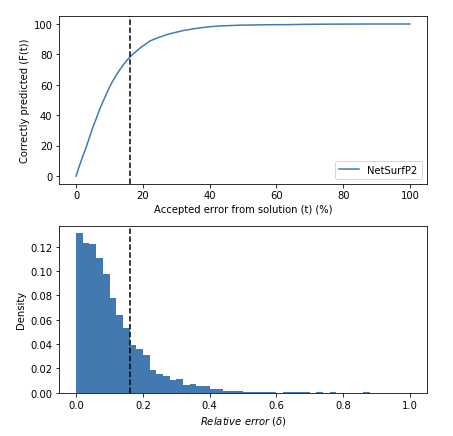
\includegraphics[width=0.48\textwidth]{figures/relerrorthres.png}
  \caption{An example of the relative threshold-based evaluation metric: In this case, a threshold range from 0 to 100 percent absolute error is used to derive at the curve in the top panel. For each threshold (exemplified by the black dashed horizontal line), the ratio of correctly predicted THSAs is calculated. This ratio is the total surface area left from the threshold, divided by the total surface area.}
  \label{fig5}
\end{figure}

\section{Results}
In this reseaurch, MolPatch was created to obtain the LHPSA as a value to predict. Two different methods are analyzed for identifying hydrophobic patches using structural protein information as input: an atom-based and a residue-based approach. The fraction of protein interaction sites of different sized patches were analyzed to find biological relevance. After this, the LHPSA obtained with MolPatch was predicted together with the THSA and RHSA. The THSA and RHSA were benchmarked against NetSurfP2. By lack of a competitor for predicting the LHPSA, our models were benchmarked against a naive model. 

\subsection{Analysing patches from MolPatch}
A dataset with protein chains and their protein-protein interacting residues obtained from the PiSITE webserver was created to analyse the patches. In total, five proteins could not be resolved using the this dataset. Hydrophobic patches of 4250 soluble proteins were analyzed using MolPatch. The size of the largest hydrophobic patch ranges from 59 to 16686$\si{\angstrom}^2$, and averages on 1057$\si{\angstrom}^2$ for the atom-based method. On average, 26 residues were found in the largest hydrophobic patch using this method. The residue-based method had similar results with the largest hydrophobic patch ranging from 53.0 to 17744$\si{\angstrom}^2$, and averages on 1301$\si{\angstrom}^2$. Also the atom-based method found 26 residues in the largest patch on average. The number of residues in the largest patch averaged on 26 in both methods. The composition of residues in the hydrophobic patches differed a lot in both methods. This is expected since the patches obtained with the atom-based method could, in theory, contain all amino acids, while patches from the residue-based method could only contain the predefined hydrophobic amino acids. 

Also, the location of the patch on a protein between the two methods do not always agree. An example of matching and contradicting patch locations can be found in figure \ref{fig6}. Here, figure A and figure B represents the graph of protein N5-glutamine methyltransferase (PDB:1NV8A), with almost precisely overlapping the largest patches (Red) for both methods. An example where the largest patches differed in size could be found in protein GSU0716 (PDB:3BIA), represented in figures C and D. It can be seen that the location of both patches is at the same side, but the largest patch obtained with the residue-based method covers much more area.

\begin{figure}[h!]
  \centering
  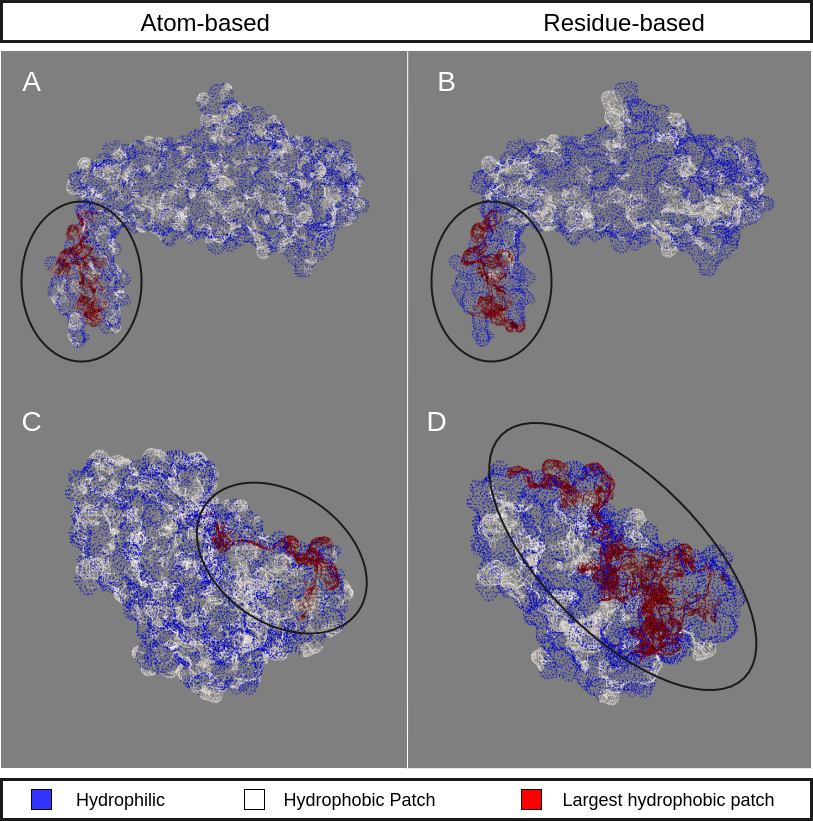
\includegraphics[width=0.48\textwidth]{figures/molpatch.png}
  \caption{This figure shows the MolPatch graphical presentation of hydrophobic patches for SabA (PDB:4O5JA) (A, B) and leishmanolysin (PDB:1LMLA) (C, D). Both atom-based (A, C) and residue-based (B, D) patch detection methods are shown. The graph consists of blue, white, and red dots representing respectively: hydrophilic sites, hydrophobic patches, and the largest patch. The largest patches are also highlighted with a circle. The largest patches in A and B show a good resemblance.  In A the size of the red area is 932$\si{\angstrom}^2$, in B it is 877$\si{\angstrom}^2$. The largest patches in C and D show a clear difference. In C the size of the red area is 583$\si{\angstrom}^2$, in D it is 2509$\si{\angstrom}^2$.}
  \label{fig6}
\end{figure}

\subsection{Interaction sites in hydrophobic patches}
The fraction of interaction sites in the top 20 largest hydrophobic patches were analyzed. In both methods, the fraction of protein interaction sites was higher in larger patches than smaller patches (table \ref{table1}). A lot of the largest patches were also found with no interaction sites at all  (S1, S2). The top 3 largest hydrophobic patches from the residue-based method got a significantly higher fraction of interaction sites than randomly expected. A significant increase was found for the top 4 protein hydrophobic patches using the atom-based method. There was also a difference in fraction protein interaction sites observed between when looked at the different rank patches. Here, a higher rank corresponds to a larger patch where rank 1 is the highest rank. The largest patch of the residue-based method contained the highest fraction of interacting site residues (0.41). This fraction has around the same value as the largest hydrophobic patch from the atom-based method (0.43). For both methods, the second-largest patch had a lower fraction compared to the largest patch (table 1). Another interesting observation is the difference between the two methods obtained fractions of protein interaction sites for lower rank patches. The fraction dropped consistently for each lower rank to a fraction of 0.1 for rank 20. This behavior was not observed using the atom-based method. The fraction dropped for the top 5 patches but stagnated around 0.22. On average, a random patch was expected to have a fraction of 0.25. The lower ranks were found to have a lower fraction of protein interaction residues than expected using the residue-based method. This was also different from the atom-based method, where all the ranks patches contained a higher fraction than were randomly expected.

\begin{table}[]
\centering
\caption{Fraction of interaction sites on hydrophobic patches}
\begin{tabular}{llll}
\hline
       & Atom-based & Residue-based & Random \\ \hline
Rank 1 & 0.43*                                         & 0.41*                                            & 0.28                                      \\
Rank 2 & 0.36*                                          & 0.33*                                            & 0.27                                      \\
Rank 3 & 0.31*                                          & 0.30*                                            & 0.27                                      \\
Rank 4 & 0.30*                                          & 0.26                                             & 0.26                                      \\
Rank 5 & 0.28                                          & 0,25                                             & 0.25                                      \\ \hline
\end{tabular}\\

\caption*{\\
The table shows the average fraction of protein-protein interacting residues in the atom-based or residue-based detected patches. Also, the fraction of interaction residues is shown for random patches. A patch is ranked in a way that Rank 1 is the largest, and rank 20 is the lowest. A * indicates $p<0.001$ obtained by the Wilcoxon test between random and atom or residue-based fractions protein interaction sites.}

\label{table1}
\end{table}

\subsection{Analyses of the THSA, RHSA, and LHPSA}
The THSA and RHSA of the 4975 monomers PDB files were estimated using DSSP. Since DSSP and NetSurfP2 are residue-based methods, the LHPSA of the same 4975 monomers dataset was determined using the residue-based method of MolPatch. The THSA values of the protein chains ranged between 288$\si{\angstrom}^2$ and 19742$\si{\angstrom}^2$. The average THSA was 3113$\si{\angstrom}^2$. The RHSA values of the protein chains ranged between 6\% and 66\%. The average RHSA was 25\%. A Pearson correlation coefficient of 0.816 was found between the length of the protein and THSA. Another obvious observation is the slight bend downwards in the curve when progressing to a longer sequence length (Figure \ref{s3}S). This bend can be explained because the surface area does not linearly correlate to molecular weight. There is no correlation found between the sequence length and the RHSA. The Pearson R for this was -0.134. The LHPSA values of the monomers ranged between 68$\si{\angstrom}^2$ and 17159$\si{\angstrom}^2$. The average LHPSA was 1248$\si{\angstrom}^2$. No correlation was found between the THSA and LHPSA, or RHSA and LHPSA.

% \begin{figure}[h!]
%   \centering
%   \includegraphics[width=0.48\textwidth]{figures/fig7.png}
%   \caption{The THSA and RHSA of a protein is plotted against its sequence length in a 2d histogram. The surface of the plot is divided where a brighter color indicates a higher concentration of proteins with values corresponding to the surface of the bin.}
%   \label{fig7}
% \end{figure}

\subsection{Prediction of THSA, RHSA, and LHPSA}
For predicting the THSA, NetSurfP2 outperformed all the simple models. The combination model of GFM and NetSurfP2 did not provide a better model. As can be seen in figure \ref{predictfig}A, the combination model followed the same curve as NetSurfP2. The GFM is the best performing model when leaving out NetSurfP2. The naive model is surprisingly well-performing compared to the GFM, which only performs a little bit better than the naive model.

\begin{figure}[h!]
  \centering
%   \captionsetup{width=.5\linewidth}
  \subfloat[]{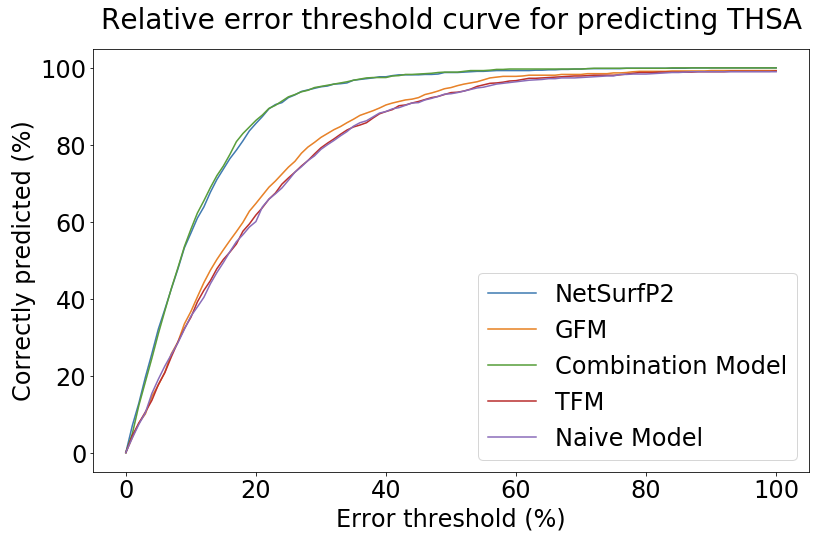
\includegraphics[width=0.48\textwidth]{figures/THSA_REAL.png}\label{fig:f1}}\\
  \subfloat[]{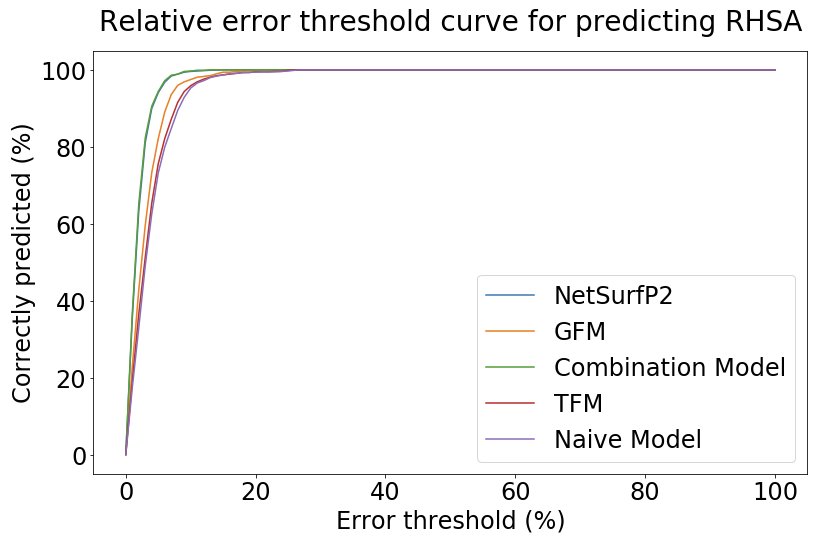
\includegraphics[width=0.48\textwidth]{figures/RHSA_REAL.png}\label{fig:f2}}\\
  \subfloat[]{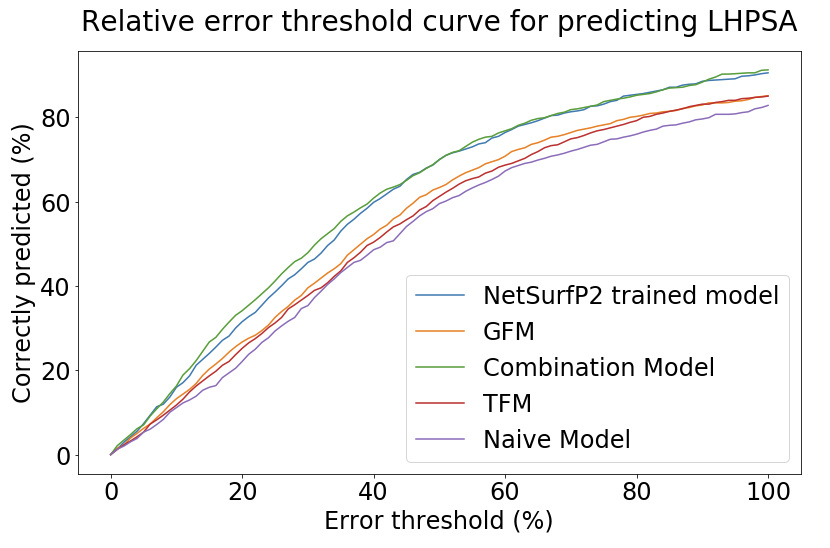
\includegraphics[width=0.48\textwidth]{figures/LPHSA_REAL.png}\label{fig:f3}}
  \caption{The relative error threshold curve in A, B, and C shows the percentage correctly predicted THSA, RHSA, and LHPSA for all proteins in the test set, given the allowed error margin. For every predictor, the combination model and NetSurfP2 obtained the highest accuracy according to the relative error threshold curve. Note that the curve shapes of figure B are different because of the different calculations for $\delta_{RHSA_i}$.}
  \label{predictfig}
\end{figure}

The RHSA is best predicted by NetSurfP2 (figure \ref{predictfig}B). The combination model gave the same prediction accuracy of the RHSA as NetSurfP2. The GFM model is still the best model when leaving out NetSurfP2 prediction. Again the naive model is slightly worse than the GFM model. When comparing the models in their performance, the same trend is shown where NetSurfP2 is performing much better. The curves have different shapes, but this does not mean that RHSA is easier to predict. The RHSA is already a percentage which resulted in a different $\delta_{RHSA_i}$ calculation compared to $\delta_{THSA_i}$.

The prediction results of the LHPSA determined by the residue-based method is shown in figure \ref{predictfig}C. The LHPSA is harder to predict compared to THSA. The NetSurp2-trained model,  which was trained with the THSA, RHSA and TASA predicted by NetSurfP2, was the best performing model for prediction of the LHPSA. Almost no difference is observed between the combination model and the NetSurfP2 model. The GFM model was the best performing model when NetSurfP2 data was omitted. All models performed much better than the Naive length-based model.

\subsection{Top 10 important global features for predicting THSA, RHSA and LHPSA using GFM}
The GFM had the highest accuracy for predicting the  RHSA and THSA when excluding NetSurfP2 results. NetSurfP2 features were also the most important for the combination model. This is why this model was chosen for examining the feature importance for THSA and RHSA. The feature importance of the GFM is indicated with a fraction. The larger value indicates a more significant predictive importance. The feature importance when predicting the LHPSA was examined for the combination model. This is because the LHPSA could not be directly obtained from NetSurfP2 data. 

The hydrophobic count (hydr\_count), buried, and length were the most predictive features for THSA prediction. Out of the amino acid counts, the hydrophobic leucine was the most predictive. The second most predictive amino acid was serine, which is polar. The following amino acid types had around the same amount of predictive power. 

The polar count (polar\_count), gravy, and aromaticity were the most predictive compound features for RHSA prediction. The most predictive amino acid was lysine. The second most predictive amino acid was serine. Methionine, valine, leucine, and glycine were the other high scoring amino acid. All of them are hydrophobic amino acids. 

The gravy index was the most predictive global features for LPHSA prediction. The most predictive amino acids were the hydrophobic phenylalanine and isoleucine. All successive amino acids in the list were equally essential.

\begin{figure*}[!tbp]
  \centering
  \captionsetup{width=.9\linewidth}
  \subfloat[]{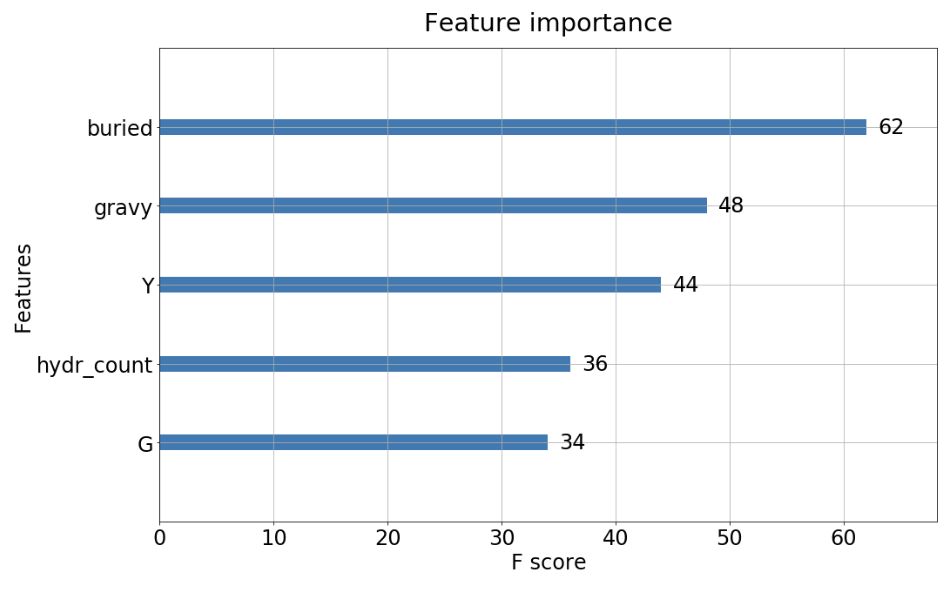
\includegraphics[width=0.31\textwidth]{figures/THSA_FIREAL.png}\label{fig:f1}}
  \subfloat[]{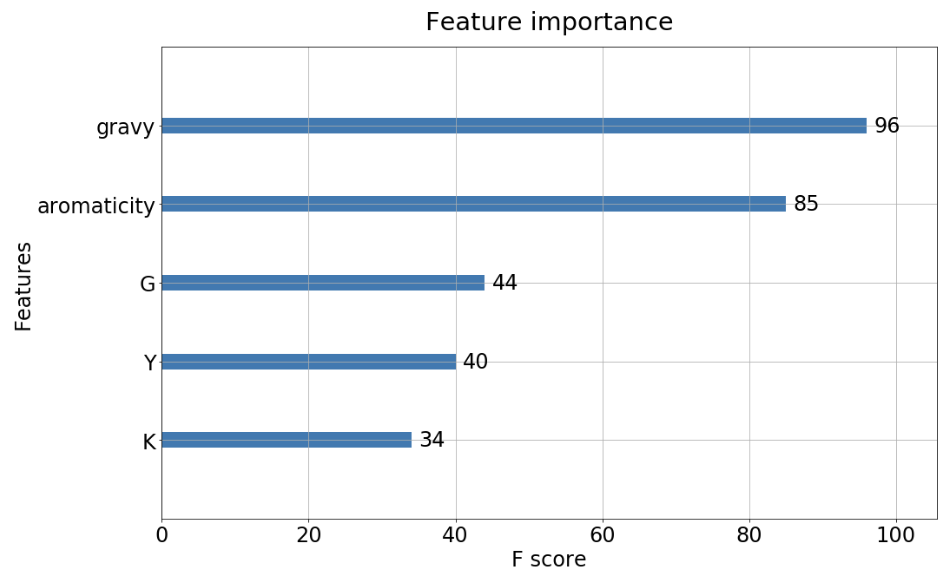
\includegraphics[width=0.31\textwidth]{figures/RHSA_FIREAL.png}\label{fig:f2}}
  \subfloat[]{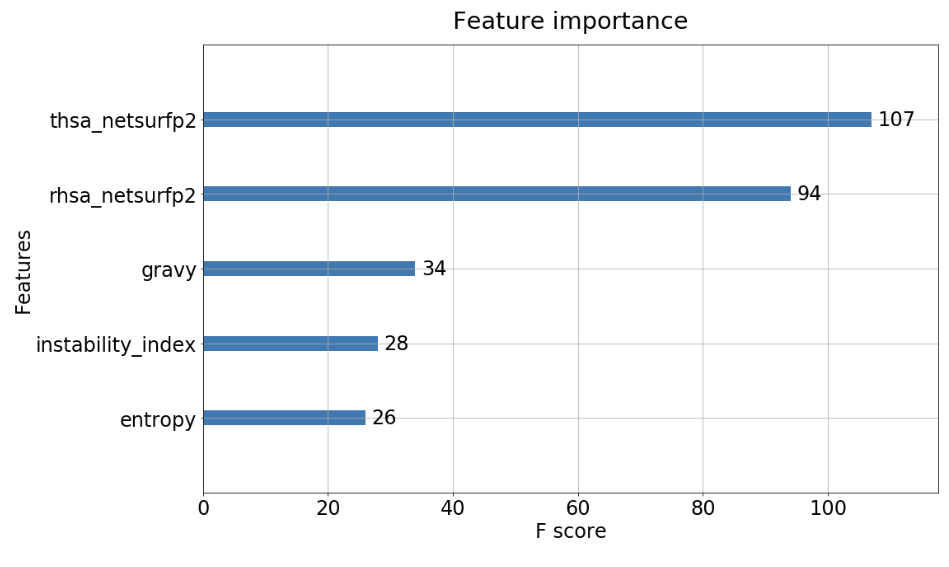
\includegraphics[width=0.31\textwidth]{figures/LHPSA_FIREAL.png}\label{fig:f3}}
  \caption{ This figure shows horizontal bar charts with the feature importance as fractions. The top 10 global sequence features for predicting THSA are shown. The top 10 predictive features for THSA were: Hydrophobic count, buried, length, leucine, serine, isoleucine, phenylalanine, threonine, glutamine, and arginine. The top 10 predictive features for RHSA were: Polar count, gravy, lysine, aromaticity, serine, length, methionine, valine, leucine, and glycine. The top 10 predictive features for LHPSA were: Gravy, buried, isoleucine, phenylalanine, hydrophobic count, length, buried, lysine, tyrosine, cysteine, and instability index.}
\end{figure*}

\section{Discussion \& Conclusion}
In this research, we have set out to answer the following questions. First, is it possible to improve the prediction of THSA and RHSA from sequence only? Second, is it possible to predict the LHPSA from sequence only?

\subsection{Biological relevance of larger patches}

No gold standard does yet exists for the largest hydrophobic patches, and it is undoable to inspect more than 4000 proteins for hydrophobic patches manually. The higher fraction of interacting residues in the largest patches found using both methods indicated the biological relevance of large hydrophobic patches. Also, a significant difference in the fractions of interacting residues is found in the higher-ranked patches when compared to lower-ranked patches. This difference agrees with the idea that large hydrophobic patches are not located on the surface by random and have a molecular function. The fraction of protein interaction sites in the largest patch obtained by the atom-based method was slightly higher than the one from the residue-based method. The better score for the atom-based method makes it plausible that this method is a better way to determine hydrophobic patches. Both methods obtained a significant higher fraction of protein interaction sites compared to random in the largest patches, which makes them both worth do be analyzed in-depth.

\subsection{Difference MolPatch and other techniques}

Quilt and the method from Eisenhaber and Argos are two other methods for the analyses of hydrophobic patches. The two methods are nearly identical with a small difference in the recovery of lost hydrophobic surface as a result of the expansion of the van der Waals radius of hydrophilic atoms. Quilt tries to correct for this while Eisenhaber and Argos' method doesn't. 

When Philip Lijnzaad's Quilt is compared to MolPatch there are two main differences in the method. The first one is the ability to use the residue-based method with MolPatch, and the second is the difference in correction for hydrophobic surface channels. Quilt uses the expansion of the van der Waals radius of hydrophilic atoms to reduce the amount of channels. MolPatch removes channels if only one of the two nearest atoms is hydrophobic. The results of MolPatch and Quilt are quite different. The main reason for this is the large difference in the size of the dataset. In a study where Quilt was used to analyse the LHPSA of 112 soluble monomeric proteins, an average of 400$\si{\angstrom}^2$ was found. This study found an average of 1057$\si{\angstrom}^2$ for 4975 proteins. In a study where Quilt descovered hydrophobic patches are analysed for interaction sites, it was found that the largest or second largest patch was 90\% percent of the time involved in multimeric interfaces. MolPatch largest two patches were only involved in 72\% of the cases. Again, the dataset size differed a lot. Quilt used a dataset of 59 proteins compared to a dataset of 4255 protein used for the analyses of interfaces using and MolPatch. Although the difficult comparison, the differences between Quilt and MolPatch show that it might be relevant to investigate a stricter channel cutoff correction for MolPatch.   

\subsection{Difference between atom-based and residue-based patch detection}

When the residue and atom-based methods were compared to each other, a couple of things stood out. First of all, the size of the largest patches in the residue-based method was more than 200$\si{\angstrom}^2$ larger. This can be explained through the different assignment of surface area to a patch. For the atom-based method, the surface of only the unique atoms in a patch was summed. The residue-based method summed the ASA of the whole residue. This could also mean that surface area was added while it was not adjacent to the patch. The residue method is therefore prone to unwanted added surface area, which might be the reason why the average ASA for the largest patch is higher using the residue-based method.

Another noticeable difference was the fraction of protein interaction sites for rank 20 in the atom and residue-based method. These values differed more than 0.15. A possible explanation is the difference in the total number of patches for this rank. Atom-based residues found a lot more patches since an atom can be a patch on itself. With the residue-based method, only entire residues were allowed in the patch. This means that if there are only five hydrophobic residues located on the surface, a maximum of 5 hydrophobic patches could be made. 
	
\subsection{Future improvements of MolPatch}

Both methods have their shortcomings, which can be improved in future studies. We proposed a new method for the removal of channels in the atom-based approach. This method included the removal of edges between surface points by analyzing the hydrophobicity of the two closest atoms. Although this method does an excellent job in closing channels, it can also remove areas close to the borders of the patch. A possible solution to solve the loss of patch area would be to return removed edges without connecting two separate patches. The parameters of the correction method for the atom-based method could also be further analyzed. The number of closest atoms needing to be hydrophobic was chosen based on the observation of the results using a small set of proteins. 
    
Another encountered problem with the atom-based method is the rough classification of hydrophobic atoms. This rough classification says that every carbon and sulfur atom is hydrophobic, and every oxygen and nitrogen atom is hydrophilic. Although this classification does hold in many cases, there are many environments where the classification should be more sophisticated. One example is the carbon atom of the carboxyl group in the backbone of a protein. This atom is slightly polar. Also, electric charges of neighboring atoms can influence the polarity of a carbon atom.

The residue-based method deals with generality. In this method, only predefined residues are allowed to be located within a patch. The problem here is that residues classified as hydrophilic can still have areas that are hydrophobic. If such areas are connecting two large hydrophobic areas together, this will not be recognized. This may also be the reason why the average of the largest hydrophobic patches are larger in size using the residue-based method compared to the atom-based method.
    
In the residue-based method, binary classification of hydrophobic residues is implemented. This classification assumes that all hydrophobic residues are equally water repellent. Protein interaction site does not always have to be classified as hydrophobic if one part of the residue is hydrophilic. These residues can, in theory, still make up for the hydrophobic patch area. A problem with the residue-based method is that it does not allow these types of residues to be located in a patch. For future studies, a more refined method of classification can be useful to select a Patch. The Kyte and Doolittle scale could be implemented for this task. The MolPatch eventually creates networks of adjacent residues. Networks with The Kyte and Doolittle scale weights attached to its nodes could then be split into distinct components using community search algorithms.  The downside of this method is the complexity and, therefore, its computation time.

\subsection{Improvement of NetSurfP2}
Robbin Bouwmeester showed in his master thesis an improved prediction compared to the best performing methods back in 2015. NetSurfP1 was one the methods the TFM was benchmarked against. The results of the TFM were a lot better compared to the results of NetSurfP1 back then. Compared to the results of NetSurfP2, we can see that NetSurfP2 has improved a lot compared to NetSurfP1 on the prediction of the THSA and RHSA.  

\subsection{No improvement of the THSA and RHSA prediction}
We have shown that NetSurfP2 has an excellent performance when predicting the THSA and RHSA of a protein. NetSurfP2 has a remarkable performance increase compared to the naive length-based model. The GFM performed slightly better than the naive based model, indicating that a more sophisticated such as NetSurfP2 is needed to get a better result when predicting THSA or RHSA. The most informative features of the GFM were instability factor and gravy. These values are logical estimators since they incorporate hydrophobicity characteristics. The top-scoring amino acid counts are mostly hydrophobic and polar amino acid types.  Neutral amino acids are found as less predictive. This makes sense since hydrophilic amino acids can have a negative influence on the THSA and RHSA, while the hydrophobic amino acids can have a positive influence.

\subsection{Predicting LPHSA with reasonable accuracy}
	
The LHPSA prediction results were slightly disappointing but compared to the THSA and RHSA results, not surprising. LHPSA prediction is far more complicated than THSA and RHSA prediction since it is unknown which residues are located in the largest patch. The GFM performed, in this case, a lot better than a naive length-based model. The most important feature was the gravy index. Isoleucine and phenylalanine were the most important amino acid for predicting the LHPSA. This makes sense because isoleucine and phenylalanine are hydrophobic and large residues. If it is located in the largest patch, it counts for a lot of surface area. In earlier studies, these two residues were also found to have a high preference to be located in larger patches [9]. The NetSurfp2 model, again,  had the best performance of all models. Overall the models show a prediction with reasonable accuracy. 

A possible next step to improve the accuracy of LHPSA is to classify which residues are located in the largest hydrophobic patch based on the amino acid sequence of a protein. This could be done in the same way as protein-protein interfaces are classified using evolutionary data [34]. The ASA of residues predicted within the patch can then be obtained using NetsurfP2 since it has proven to predict the ASA of hydrophobic residues quite accurately. Another method would be to predict the LHSPA directly from a single model with the sequence as input.


\section*{Acknowledgments}
I would like to express my gratitude to my supervisors Sanne Abeln and Juami van Gils for the help and engagement through the learning process of this master thesis. 

\bibliography{jan}
\bibliographystyle{unsrt}

\appendix

\section{Appendices}
\label{sec:appendix}

\begin{figure}[h!]
  \centering
  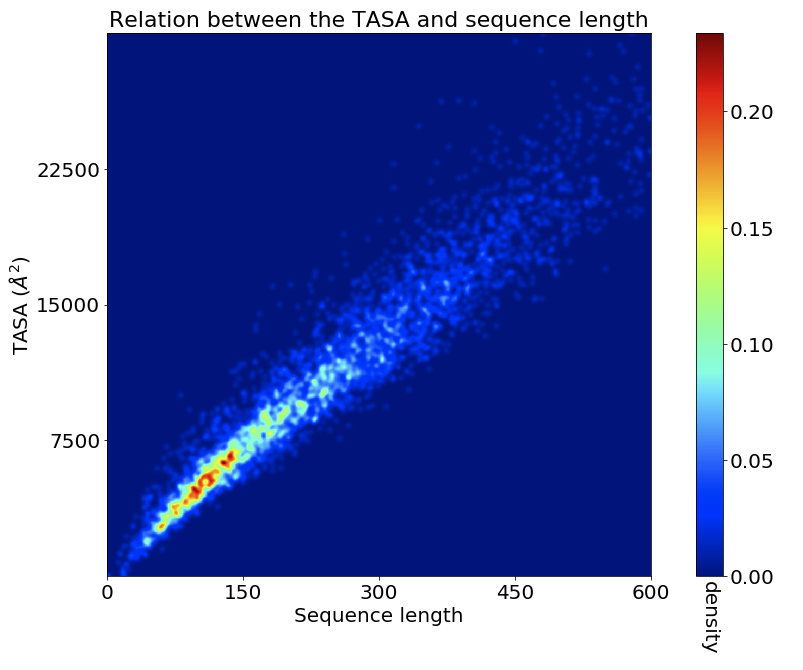
\includegraphics[width=0.48\textwidth]{figures/TASA_LENGTH.png}
  \caption{In this figure, the number of residues of a protein is plotted against the TASA in a density heatmap. A slight bend can be observed in the ranges 40-100.
}
  \label{s3}
\end{figure}

\begin{figure}[h!]
  \centering
  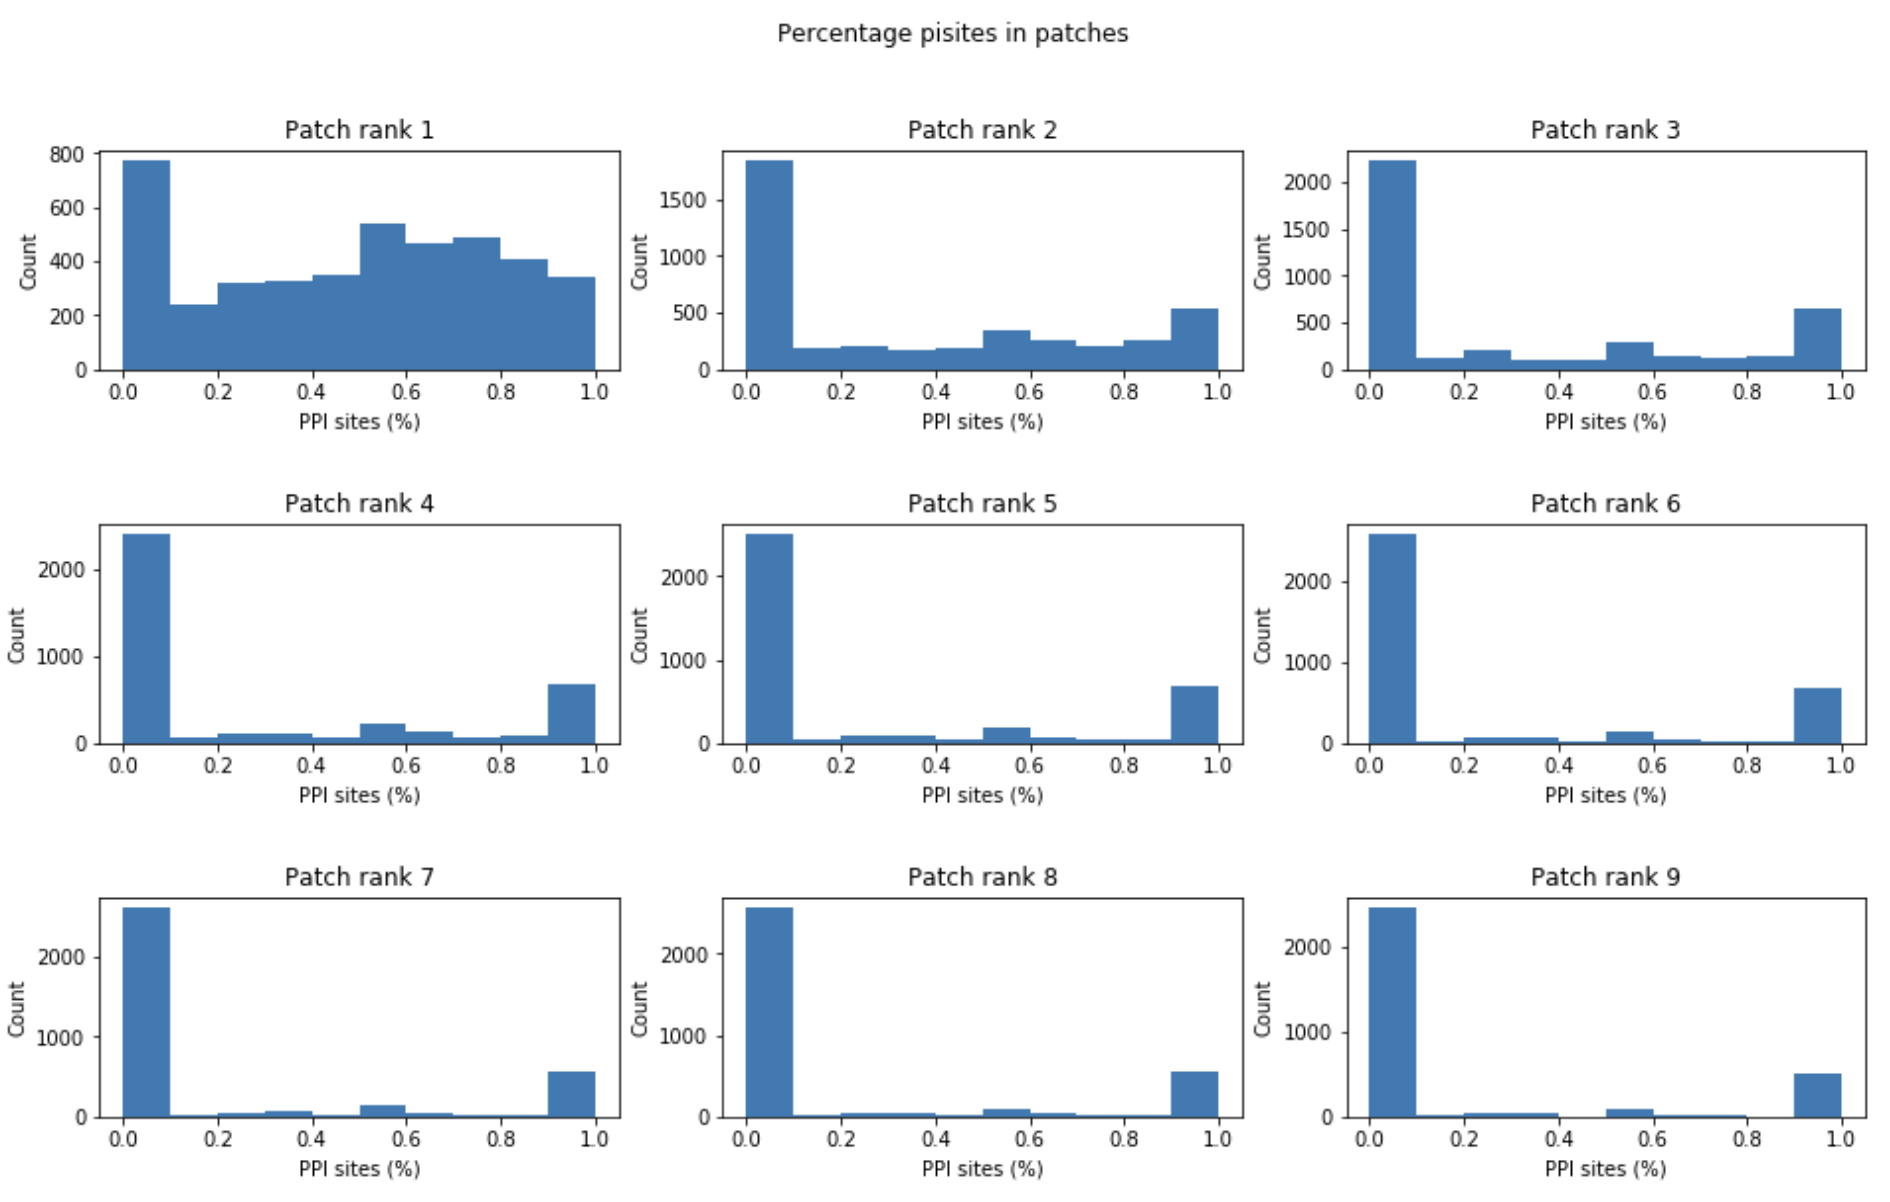
\includegraphics[width=0.48\textwidth]{figures/s1.png}
  \caption{The distribution of the fraction protein interaction sites in a patch detected by the atom-based method. Rank 1 is the largest patch and rank 9 is the 9th largest patch. This figure shows that the largest hydrophobic patch has a lot more interaction sites compared to smaller size patches.
}
  \label{s1}
\end{figure}

\begin{figure}[h!]
  \centering
  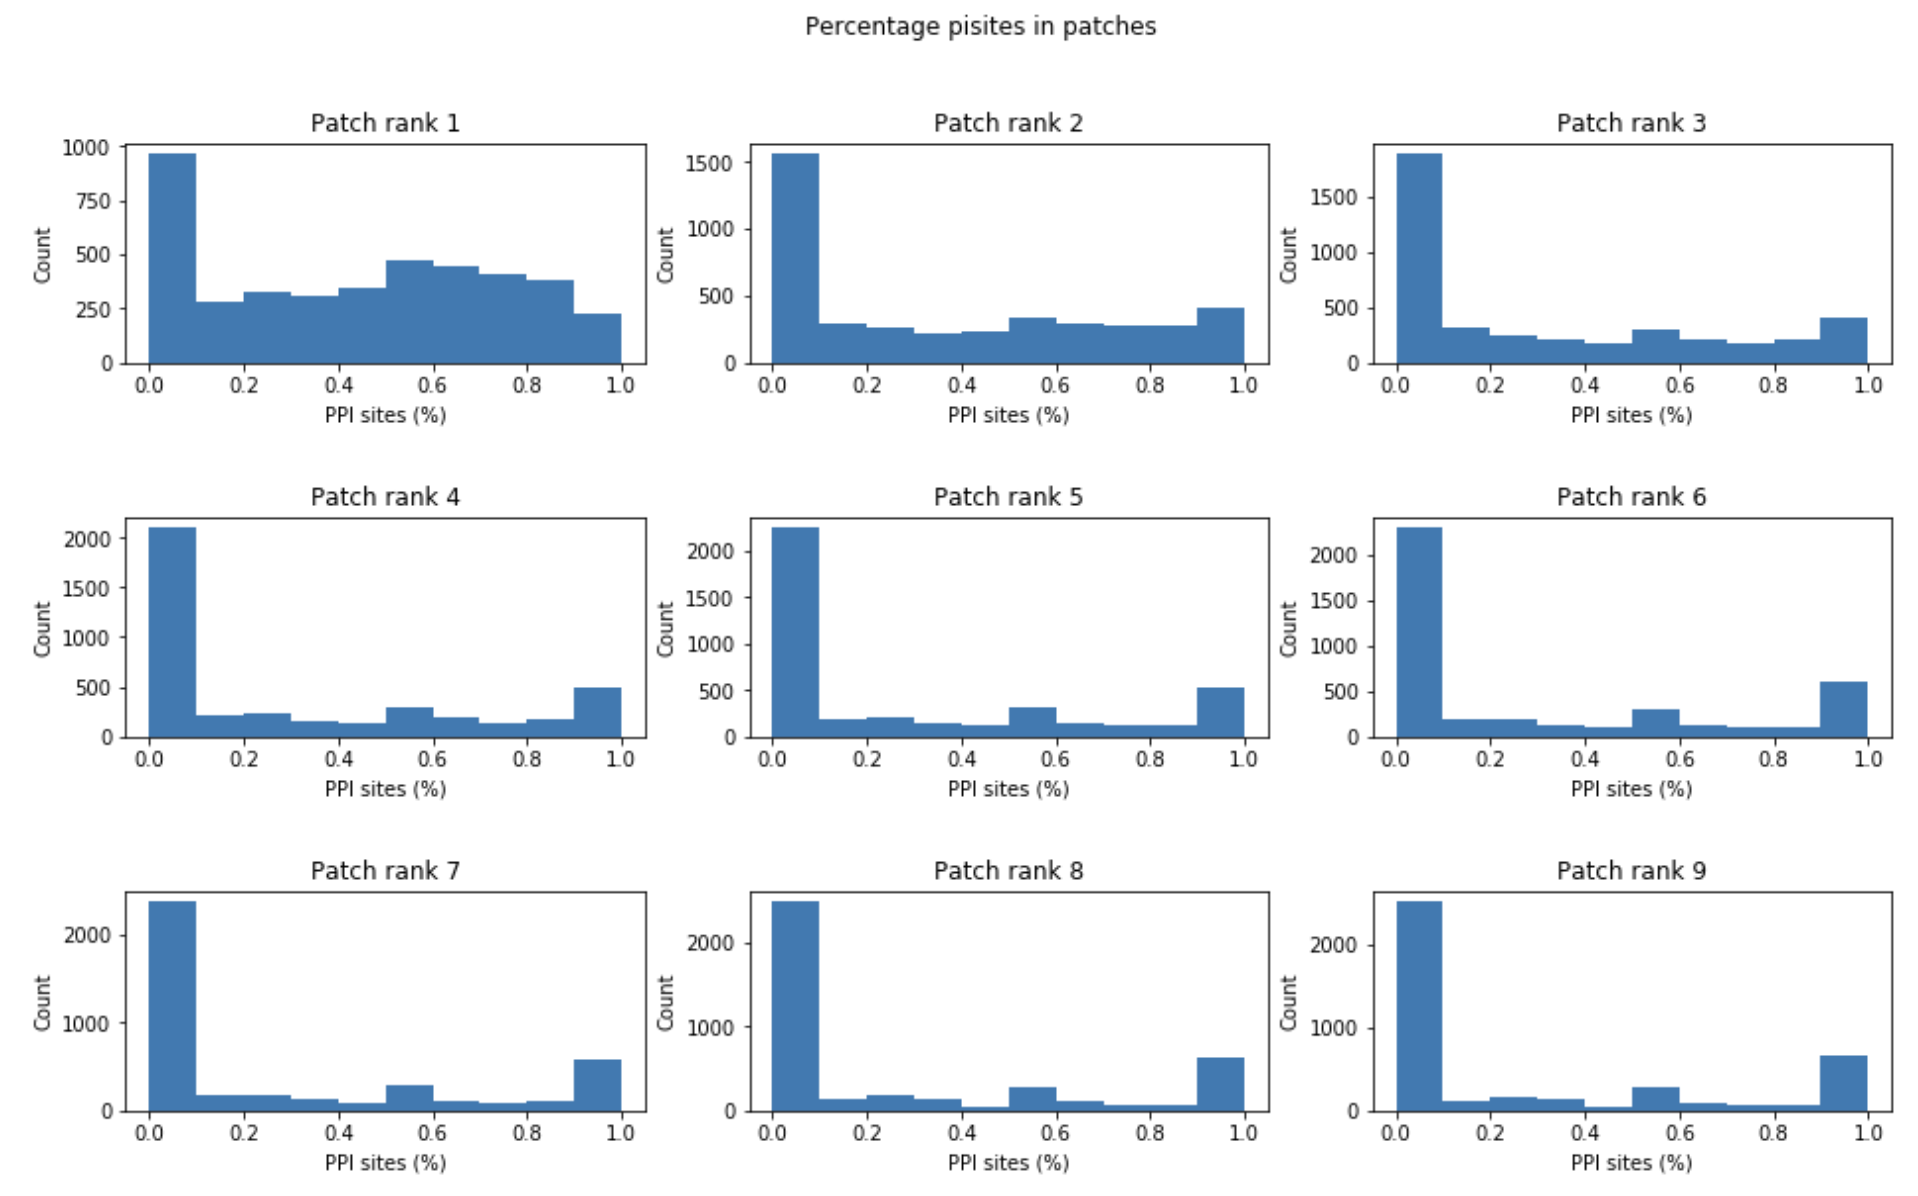
\includegraphics[width=0.48\textwidth]{figures/s2.png}
  \caption{ The distribution of the fraction protein interaction sites in a patch detected by the residue-based method. Rank 1 is the largest patch and rank 9 is the 9th largest patch. This figure shows that the largest hydrophobic patch has a lot more interaction sites compared to smaller size patches.}
  \label{s2}
\end{figure}


% \section{Supplemental Material}
% \label{sec:supplemental}
% Submissions may include non-readable supplementary material used in the work and described in the paper. Any accompanying software and/or data should include licenses and documentation of research review as appropriate. Supplementary material may report preprocessing decisions, model parameters, and other details necessary for the replication of the experiments reported in the paper. Seemingly small preprocessing decisions can sometimes make a large difference in performance, so it is crucial to record such decisions to precisely characterize state-of-the-art methods. 

% Nonetheless, supplementary material should be supplementary (rather
% than central) to the paper. \textbf{Submissions that misuse the supplementary 
% material may be rejected without review.}
% Supplementary material may include explanations or details
% of proofs or derivations that do not fit into the paper, lists of
% features or feature templates, sample inputs and outputs for a system,
% pseudo-code or source code, and data. (Source code and data should
% be separate uploads, rather than part of the paper).

% The paper should not rely on the supplementary material: while the paper
% may refer to and cite the supplementary material and the supplementary material will be available to the
% reviewers, they will not be asked to review the
% supplementary material.


\end{document}
